\chapter{Ausarbeitung des Architekturkonzepts}\label{chap:concept}
\section{Analyse und Übersetzung der bisherigen UI-Struktur}\label{sec:ui_structure_translation}
Momentan werden alle für die Darstellung der verschiedenen Ansichten benötigten Parameter und Metadaten in einzelnen Dateien als Teil des Solution-Verzeichnis gespeichert. `<Ansichtsname>.dli' enthält die Konfiguration für die Detailansicht und `<Ansichtsname>.vlc' die Konfiguration der Übersichtsliste. Für den Aufbau dieser Dateien existiert leider keine offizielle Spezifikation und auch keine Dokumentation, es ist daher eine Herausforderung direkt alle nötigen Informationen aus ihnen auszulesen und bedarf unter Umständen spätere Anpassungen am Auslesetool oder der künftigen Struktur. In diesem Abschnitt werden nur die tatsächlich benötigten bzw. ausgelesenen Informationen beschrieben.

\subsection{Detailansicht (DLI)}
Die relevanten Teile der Detailansicht bestehen aus verschachtelten \textbf{List}-Elementen. Die erste Ebene bilden die Seiten (\textbf{Page0 bis PageN}), eine verschachtelbare Gruppierung von Elementen. Jede Seite besteht aus wenigen Metadaten wie dem Name, einer Hintergrundfarbe, etc., einem \textbf{Controls}-Element und den darin enthaltenen \textbf{Control}-Elementen. Ein \textbf{Control}-Element hat einen bestimmten Typ und enthält abhängig von diesem etliche weitere Eigenschaften die typspezifisch ausgewertet werden müssen. Die grundsätzliche Form der neuen Struktur ist in Auflistung~\ref{lst:detailview_structure} beschrieben.

\lstinputlisting[label={lst:detailview_structure},caption={Datentypen der neuen Detailansicht-Struktur}]{code/chapter_004_detailview_structure.txt}

\subsection{Übersichtsliste (VLC)}
Im Vergleich zur Detailansicht ist der Aufbau der Übersichtsliste simpler. Es existieren eine oder mehrere \textbf{List}-Elemente, welche wiederum eine beliebige Anzahl an \textbf{Column}-Elementen enthalten können. Ein Listenelement und die enthaltenen Spalten gehören zu einer bestimmten Datenbanktabelle, diese Information muss also zusätzlich zum Spaltennamen gespeichert werden. Die Form der neuen Struktur ist analog zur Beschreibung der Detailansicht in Auflistung~\ref{lst:listview_structure} zu sehen.

\lstinputlisting[label={lst:listview_structure},caption={Datentypen der neuen Übersichtslisten-Struktur}]{code/chapter_004_listview_structure.txt}

\subsection{Neue Struktur}
Die neue generierte Struktur entspricht dem initialen Zustand der neuen UI und enthält neben den ausgelesenen Elementen und deren Formatierung auch Informationen für die Darstellung des Layouts. Die hierfür gespeicherten Informationen entsprechen dabei denen von den Layout-Bibliotheken (siehe Abschnitt~\ref{subsec:layout}) generierten Serialisierungen. Das bedeutet, dass weder auf dem Client noch auf dem Server Sonderfälle für die `erste' (bevor der Nutzer die Anzeige individualisiert) Darstellung notwendig sind --- die Datenstruktur ist identisch, ob es sich um den initialen oder einen angepassten Zustand handelt ist für Client und Server also vollkommen transparent.

\section{Webseite}
Zum jetzigen Zeitpunkt muss die Clientapplikation nur eine einzige Ansicht des \gls{crm} darstellen können. Hierzu wird ein Projekt mit einer Hauptkomponente und zwei weiteren Komponenten für die Übersichtsliste und die Detailansicht erstellt. Die Hauptkomponente zeigt je nach Auswahl entweder die Listen- oder die Detailkomponente an. In diesen Komponenten wird die Darstellungsstruktur vom Server abgefragt und mit dieser Antwort vorgefertigte UI-Komponenten dynamisch platziert. Bei externen Änderungen der Daten wird dieser Vorgang mithilfe von GraphQL-Abonnements (siehe Abschnitt~\ref{subsec:graphql}) wiederholt und die UI somit aktualisiert.

\subsection{React-Komponenten}
Die jetzige Oberfläche besteht aus einer festen Anzahl von Darstellungs-Elementen welche je nach Kontext andere Inhalte anzeigen. Zu den Elementen gehören unter anderem statische Texte, Eingabefelder, Check- und Comboboxen, Gruppierungen und Container für weitere Elemente. Der Kontext für den Inhalt ergibt sich aus dem Datenbankfeld das mit dem jeweiligen Element verknüpft ist und Einstellungen wie Sichtbarkeitsbedingungen oder Formatierungen. Da bereits im Voraus bekannt ist, welche Art von UI-Elementen benötigt werden, können diese auch schon im Vorfeld erstellt werden. Diese fertigen \nameformat{React}-Komponenten werden mit dem Produkt ausgeliefert und können zur Laufzeit dynamisch auf der Webseite platziert werden. Die Funktionalität dieser Elemente orientiert sich dabei immer an der Funktionalität der Originalkomponente.

\subsection{Komponenten-Layout}
Für die sinnvolle Nutzung der vorgefertigten Komponenten ist es notwendig, diese nicht nur einfach nacheinander auf der Seite zu platzieren, sondern ein bedienbares Layout für die Platzierung anzubieten. Die Umsetzung wird in diesem Abschnitt dargelegt.

\subsubsection{Erste Überlegungen}
Zu Beginn erschien die zentrale Frage, wie es technisch möglich ist, die Komponenten der Detailansicht vom Benutzer anpassbar anzuordnen. Eine naive Herangehensweise kann in Abbildung~\ref{fig:layout_grid_test} gesehen werden. Umgesetzt wurde dies mit einem CSS-Grid (rote Umrandung) das entweder horizontal oder vertikal in zwei Hälften getrennt werden kann. Jede dieser Hälften stellt abermals ein CSS-Grid dar das beliebig zwischen Elterncontainern verschoben werden kann. Es handelt es sich bei diesem Ansatz um eine binäre Baumstruktur an dessen Endpunkten (Blätter) sich eine Liste von UI-Komponenten (blaue Umrandung) befindet. Durch den sich davon unterscheidenden Aufbau der Desktop-UI ist es schwierig eine simple Abbildung von der einen auf die andere zu finden. Lösungen wären vermutlich komplex und zeitaufwändig, daher wurde dieser Ansatz gänzlich verworfen und nach einer Alternativen Lösung gesucht.

\begin{figure}
    \centering
    \captionsetup{justification=centering}
    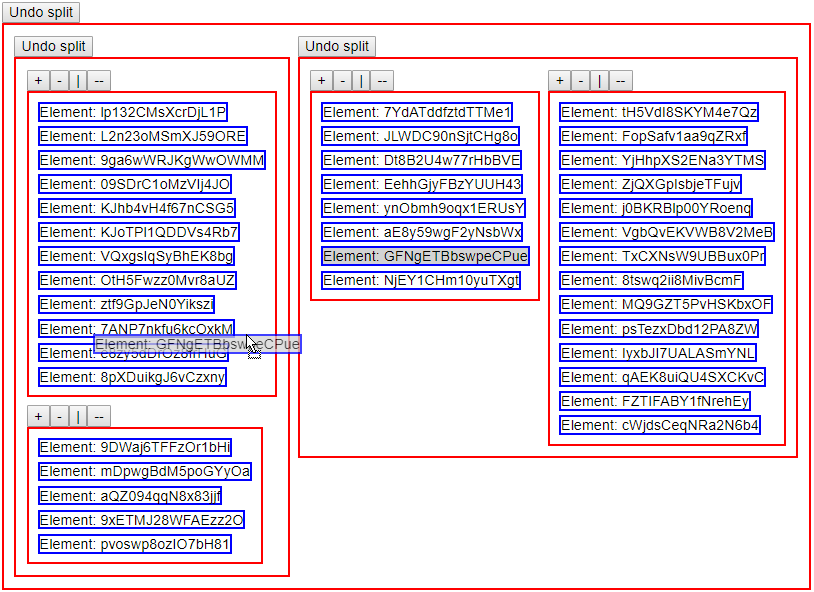
\includegraphics[width=0.8\textwidth]{figures/layout_grid_test.png}
        \caption{Eigener Layout-Prototyp mit CSS-Grids}\label{fig:layout_grid_test}
\end{figure}

\subsubsection{Umsetzung}\label{subsec:layout}
\fixme{content} % table / grid

\subsection{Identifikation auf Server}
Um die UI-Elemente mit Daten aus der Datenbank zu befüllen muss eine entsprechende Identifikation möglich sein. Es wird vorausgesetzt dass diese eindeutige ID, ob sie aus Tabellennamen plus Spaltenname der Datenbank oder aus anderen Informationen besteht, zum Zeitpunkt der Übersetzung einer Ansicht bereits bekannt ist und mit ausgelesen werden kann. Bei Anfragen an den Server werden alle IDs der beteiligten Elemente mit an den Server übertragen, ebenso wie dieser bei Antworten immer die IDs der Elemente, für welche die Antwortdaten gedacht sind, sendet.

\subsection{Visualisierung von Lade- und Fehlerzustände}\label{subsec:loading_state_section}
Direktes Feedback ist für die subjektive Einschätzung einer performanten Webseite essentiell. Typischerweise ist die am längsten dauernde Aktion auf einer Webseite das Nachladen von Daten, es ist also sinnvoll diesen Vorgang für Nutzer visuell ansprechend deutlich zu machen. Für diesen Zweck sollen alle \nameformat{React}-Komponenten eine visuell simplere Repräsentation von sich selbst in Form von unspezifischen grauen Boxen enthalten, welche nur auf die ungefähre Form und Darstellung mit Echtdaten hindeutet und die bereits während des Ladevorgangs angezeigt werden kann. In Abbildung~\ref{fig:comp_loading_final_comparison} sieht man eine Gegenüberstellung der beiden Repräsentationen (finaler Zustand links, Ladezustand rechts), jeweils für ein Edit-Element und ein Checkbox-Element.

\begin{figure}
    \centering
    \captionsetup{justification=centering}
    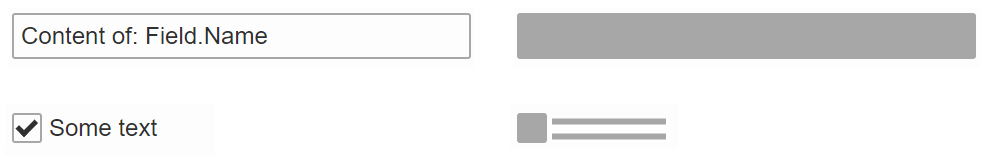
\includegraphics[width=\textwidth]{figures/comp_loading_final_comparison.png}
        \caption{Ladezustand einer Komponente}\label{fig:comp_loading_final_comparison}
\end{figure}

Mit einer entsprechende Einfärbung und einem Hinweistext kann diese Visualisierung, wie in Abbildung~\ref{fig:comp_possible_error_state} an zwei unterschiedlichen Ausführungen gezeigt, ebenfalls dazu genutzt werden um Fehlerzustände beim Laden von Daten zu signalisieren.

\begin{figure}
    \centering
    \captionsetup{justification=centering}
    
\includegraphics[width=0.8\textwidth]{figures/comp_possible_error_state.png}
        \caption{Mögliche Fehlerzustände einer Komponente}\label{fig:comp_possible_error_state}
\end{figure}

\subsection{Einbindung von GraphQL mit Apollo}
Um \nameformat{Apollo} mit \nameformat{React} zu nutzen, muss zu Beginn einmalig die Adresse des Servers einer \textbf{Apollo-Provider}-Komponente übergeben werden. Diese umschließt alle weiteren Komponenten und dient dazu die Serveradresse an jeder Stelle der App zur Verfügung zu stellen. Zum Abfragen von Daten für die Darstellung in einer Komponente wird eine spezielle Funktion mit der \nameformat{GraphQL}-Abfrage, der daraus resultierenden Datenstruktur und der eigentlichen Komponente konfiguriert. Der Rückgabewert dieser Funktion verhält sich identisch zur übergebenen Komponente, enthält aber zusätzlich noch die aus der Abfrage erhaltenen Daten (und ggf. Lade- / Fehlerinformationen) als Übergabeparameter und kann diese identisch zu lokalen Daten bei der Anzeige nutzen.
Dieser Ansatz erlaubt es, die \nameformat{GraphQL}-Abfragen komponentenspezifisch (jede Komponente ist für den Aufbau der für sie notwendigen Abfrage zuständig) zu schreiben und lokal in einer zugehörigen Datei `<Komponentenname>.gql' zu speichern. Änderungen oder ein Austausch von Komponenten sind durch diese lose Kopplung der einzelnen Teile der Applikation trivial, da sie nur eine geringe Auswirkung auf alle anderen Komponenten haben.

\subsection{Unveränderbare Daten}
Das Verwalten von Mutationen mit veränderbaren Daten ist schwieriger, je größer ein Projekt wird, da diese immer in allen Teilen des Programms ausgeführt werden müssen. Durch Programmierfehler kann es passieren, das bestimmte Änderungen eventuell nicht überall vollzogen werden und so der State nicht mehr synchronisiert ist. Um diese Art von Fehler zu verhindern werden Daten nur an einer zentralen Stelle verwaltet (\textbf{single source of truth}) und sind an allen anderen Stellen unveränderbar (\textbf{immutable data}). Mutationen werden als Aktion an die für die Daten verantwortliche Stelle gesendet und nacheinander abgearbeitet.

\subsection{Editier-Modus}
In der UI angezeigte Daten kommen direkt vom Server und werden vor der Anzeige nicht weiter verarbeitet (siehe Abschnitt~\ref{subsec:api_client_no_business_logic}). Aufgrund dieser Tatsache kann eine Kopie des zu editierenden Objekts erstellt und Änderungen auf dieser Kopie ausgeführt werden. Wird der Editier-Modus durch Verwerfen der Änderungen beendet, so muss nur diese Kopie gelöscht werden. Andernfalls wird das Original durch die Kopie ersetzt und der Server über die Mutation benachrichtigt. Dieses Konzept wird von der Bibliothek \nameformat{immer.js} \parencite{weststrate_2019} umgesetzt und anhand einer Grafik (\ref{fig:immer_draft_concept}) sehr anschaulich dargestellt.

\begin{figure}
    \centering
    \captionsetup{justification=centering}
    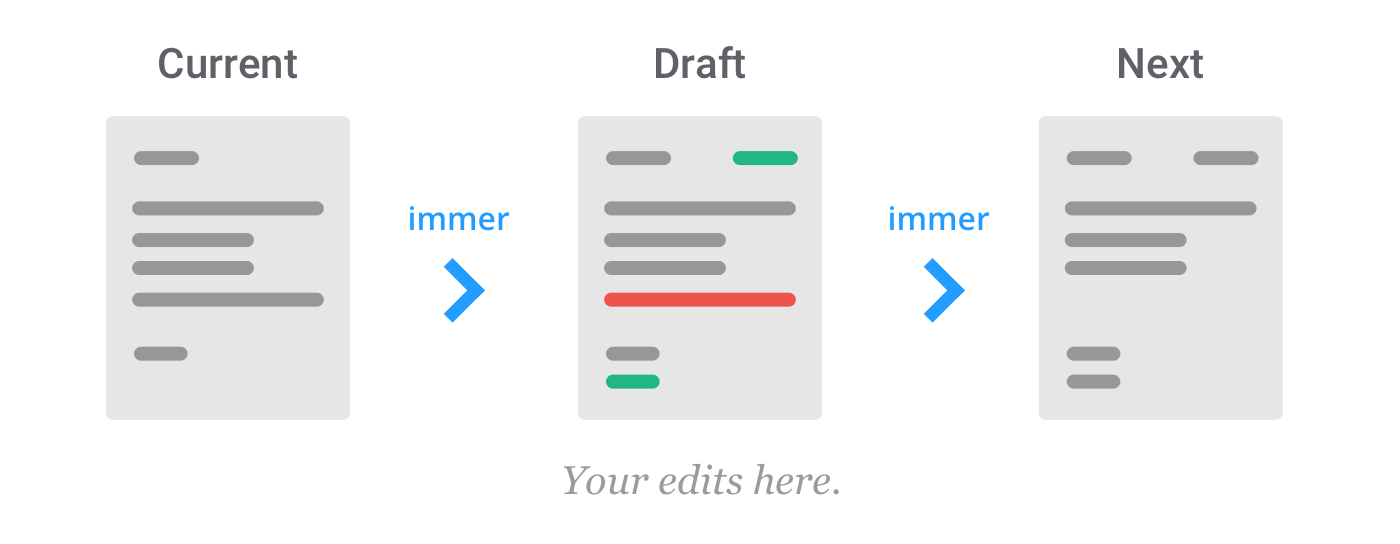
\includegraphics[width=\textwidth]{figures/immer_draft_concept.png}
        \caption{Editier-Konzept von immer.js \parencite{weststrate_2019}}\label{fig:immer_draft_concept}
\end{figure}

\subsection{Individualisierung}
Die Serialisierung des Layouts nach JSON geschieht über die jeweilige Darstellungsbibliothek der Ansicht. Zusätzliche (eigene) Formatierungen aus der Detailansicht werden anschließend im JSON ergänzt und dann auf den Server übertragen. Bevor das erste Mal eine solche Anpassung der Ansichten vorgenommen wird entspricht die Darstellung dabei der in Abschnitt~\ref{sec:ui_structure_translation} beschriebenen, aus der Desktop-UI automatisch generierten Struktur. Das Backend kann diese Informationen entweder direkt als Datei oder in einer NoSQL-Datenbank als Dokument abspeichern, oder seinerseits eine Serialisierung in bestehende SQL-Datenbankschemas vornehmen. Zur Darstellung werden diese Informationen wie in Abschnitt~\ref{subsec:grapql_schema} dargestellt wieder vom Server abgerufen.

\subsection{Suche, Filter, Sortierung}
Die Darstellung der Übersichtsliste wird, wie oben beschrieben, die \nameformat{React}-Bibliothek \nameformat{\fixme{name aus layout section oben}} (siehe Abschnitt~\ref{subsec:layout}) benutzt. Diese ermöglicht das Suchen, Filtern und Sortieren bereits ohne weitere Anpassungen. Für die Detailansicht müssen im jetzigen Stand analog zum Desktopclient die vorhandenen Möglichkeiten im Backend zur Umsetzung der Suche und Filter genutzt werden. Ein Nachteil dieses Ansatz ist natürlich, dass jedes Mal eine Anfrage an den Server geschickt werden und alle (gefilterten) Daten neu übertragen werden müssen. Eine bessere Alternative bestünde darin, die Daten der Detailansicht ebenfalls durch \nameformat{\fixme{name aus layout section oben}} verarbeiten zu lassen --- die technische Umsetzbarkeit bedarf weiterer Analysen der Bibliothek.

\subsection{Tests und Continuous Integration}\label{subsec:test_ci_concept}
Boilerplate-Projekte welche mit dem \gls{cli}-Tool \nameformat{\gls{cra}} erstellt werden sind bereits so konfiguriert, dass gewöhnliche Tests (mit dem Testframework \nameformat{Jest}) direkt ausgeführt werden können. Entsprechende Tests sollen dabei entweder schon vor dem Hinzufügen neuer Funktionalitäten oder mindestens parallel dazu stattfinden. Zusätzlich wird noch die Bibliothek \nameformat{Enzyme} genutzt, welche \nameformat{React}-Komponenten mit einer beliebigen Verschachtelungstiefe in eine Variable rendern und dadurch in Kombination mit Jest sogenannte Snapshot-Tests ausführen kann. Bei dieser Art von Test werden die Komponenten in eine JSON-ähnliche Struktur serialisiert und diese Struktur im Dateisystem gespeichert. Bei jeder weiteren Ausführung werden die alte und die neue Struktur miteinander verglichen und der Test als fehlgeschlagen gewertet, sobald die Strukturen Unterschiede enthalten. Mit dieser Art von Test kann sichergestellt werden, dass Änderungen an der Logik keine visuellen Artefakte generieren. Alle normalen und die beschriebenen Snapshot-Tests können im Sinne der kontinuierlichen Integration\footnote{CI: Continuous Integration} auf dem internen \nameformat{Team City}-Server ausgeführt werden.
Neben diesen Tests wird während der Entwicklung und Anpassung der UI das Tool \nameformat{Storybook} genutzt, mithilfe dessen eine \nameformat{React}-Klasse isoliert von allen anderen Klassen angezeigt werden kann, genutzt. So ist es möglich, eine interaktive Echtzeit-Darstellung von Änderungen am Code zur direkten Beurteilung der gewünschten Auswirkungen zu nutzen.

\section{API}
\fixme{more infos?}

\subsection{Aufbau / GraphQL-Schema}\label{subsec:grapql_schema}
Das Schema, welches den Aufbau der Anfragen und damit gleichzeitig der Antworten vorgibt, enthält zwei Einstiegspunkte. Zum einen können Informationen zur Übersichtsliste und zum Anderen die der Detailansicht abgefragt werden. Beide Zweige sind weiterhin in eine Struktur- und einen Datenabschnitt getrennt. Clients können so zuerst die Struktur, also alle Enthaltenen UI-Elemente und deren Platzierung, Formatierung, etc., der Ansicht abfragen. Die reine Struktur enthält im Vergleich wenige Daten, eine entsprechende Abfrage erhält also zügig eine Antwort. Während die UI anschließend anhand der Struktur aufgebaut wird und Lade-Platzhalter (siehe Abschnitt~\ref{subsec:loading_state_section}) anzeigt können parallel die Daten nachgeladen werden. Sobald auch dieser Vorgang abgeschlossen ist werden die Lade-Platzhalter je nach Erfolg beziehungsweise Misserfolg mit den tatsächlichen Feldinhalten oder der Fehlervisualisierung inklusive Fehlermeldung ausgetauscht.

\subsection{Keine Business Logik im Client}\label{subsec:api_client_no_business_logic}
Clients sollten keine eigenen Schlussfolgerungen aus den von der API gelieferten Daten ziehen müssen. Dies ist ein häufig begangener Fehler, bei dem die API Daten zu einer Ressource angibt, diese Daten aber nicht direkt angezeigt sondern erst noch auf irgendeine Art verarbeitet und transformiert werden müssen. Es kann vorkommen, dass verschiedene Implementierungen von Clients an dieser Stelle andere Transformationen anwenden und die sichtbare Darstellung dabei für Endanwender inkonsistent erscheint. Selbst wenn darauf geachtet wird, dass zu einem Zeitpunkt X alle Clients konsistent implementiert sind ist es möglich diese Konsistenz durch Bugfixes oder andere clientspezifische Anpassungen in der Zukunft zu einem beliebigen Zeitpunkt Y wieder zu verlieren. Ein Beispiel für einen solchen Fall, beschrieben von Phil Sturgeon \parencite{sturgeon_2017}, ist eine API die Anfragen über Rechnungen beantwortet und dabei verschiedene Felder liefert. Enthält das Feld `\textbf{bezahlt-am}' keine Daten, können Clients davon ausgehen dass die Rechnung noch nicht bezahlt wurde. Wenn nun ein weiteres Feld, welches anzeigt ob der Betrag tatsächlich auf dem Empfängerkonto eingegangen ist, `\textbf{bezahlung-erhalten-am}' hinzugefügt wird, zeigen alte Clients den Status weiterhin als `Bezahlt', sobald das erste Feld einen Wert enthält. Clients die ein Update erhalten haben zeigen dieses Status jedoch erst, wenn beide Felder einen Wert enthalten.
Entsprechend ist diese API so konzipiert, dass notwendige Transformationen immer im Backend vollzogen werden. In der aktuellen Implementierung gibt es noch keine Instanz bei der dieses Paradigma angewendet werden muss, spätere Anpassungen und Ergänzungen an der API müssen aber entsprechend umgesetzt werden.
